%texexptitled======================================================================
% lab1-gcd
%-----------------------------------------------------------------------
%

\documentclass[11pt]{article}

% Package includes

\usepackage{graphicx}
\usepackage{color}
\usepackage{comment}
\usepackage{multirow}
\usepackage{askmaps}
\usepackage{amssymb}
\usepackage{amsmath}
\usepackage{tikz}
\usepackage{circuitikzgit}
\usetikzlibrary{arrows, positioning, shapes.geometric, circuits.logic.US}
\tikzstyle{line}=[draw]
\tikzstyle{arrow}=[draw, -latex]

% Wrap long URLs with hyphens
\PassOptionsToPackage{hyphens}{url}\usepackage{hyperref}
\usepackage{pdftexcmds}
\usepackage{upquote}
\usepackage{textcomp}
\usepackage{minted}
\usepackage[listings]{tcolorbox}
\usepackage{enumerate}
\usepackage{enumitem}
\usepackage{mathtools}
\DeclarePairedDelimiter{\ceil}{\Big\lceil}{\Big\rceil}

\tcbset{
texexp/.style={colframe=black, colback=lightgray!15,
         coltitle=white,
         fonttitle=\small\sffamily\bfseries, fontupper=\small, fontlower=\small},
     example/.style 2 args={texexp,
title={Question \thetcbcounter: #1},label={#2}},
}

\newtcolorbox{texexp}[1]{texexp}
\newtcolorbox[auto counter]{texexptitled}[3][]{%
example={#2}{#3},#1}

\setlength{\topmargin}{-0.5in}
\setlength{\textheight}{9in}
\setlength{\oddsidemargin}{0in}
\setlength{\evensidemargin}{0in}
\setlength{\textwidth}{6.5in}

% Useful macros

\newcommand{\note}[1]{{\bf [ NOTE: #1 ]}}
\newcommand{\fixme}[1]{{\bf [ FIXME: #1 ]}}
\newcommand{\wunits}[2]{\mbox{#1\,#2}}
\newcommand{\um}{\mbox{$\mu$m}}
\newcommand{\xum}[1]{\wunits{#1}{\um}}
\newcommand{\by}[2]{\mbox{#1$\times$#2}}
\newcommand{\byby}[3]{\mbox{#1$\times$#2$\times$#3}}


\newenvironment{tightlist}
{\begin{itemize}
 \setlength{\parsep}{0pt}
 \setlength{\itemsep}{-2pt}}
{\end{itemize}}

\newenvironment{titledtightlist}[1]
{\noindent
 ~~\textbf{#1}
 \begin{itemize}
 \setlength{\parsep}{0pt}
 \setlength{\itemsep}{-2pt}}
{\end{itemize}}

% Change spacing before and after section headers

\makeatletter
\renewcommand{\section}
{\@startsection {section}{1}{0pt}
 {-2ex}
 {1ex}
 {\bfseries\Large}}
\makeatother

\makeatletter
\renewcommand{\subsection}
{\@startsection {subsection}{1}{0pt}
 {-1ex}
 {0.5ex}
 {\bfseries\normalsize}}
\makeatother

% Reduce likelihood of a single line at the top/bottom of page

\clubpenalty=2000
\widowpenalty=2000

% Other commands and parameters

\pagestyle{myheadings}
\setlength{\parindent}{0in}
\setlength{\parskip}{10pt}

% Commands for register format figures.

\newcommand{\instbit}[1]{\mbox{\scriptsize #1}}
\newcommand{\instbitrange}[2]{\instbit{#1} \hfill \instbit{#2}}

\newif\ifsolution

\if\issolution1
\newenvironment{solution}
    {\color{red}}
    {\color{black}}
\solutiontrue
\else
\excludecomment{solution}
\solutionfalse
\fi


\graphicspath{{./figs/}}


%-----------------------------------------------------------------------
% Document
%-----------------------------------------------------------------------

\begin{document}
\def\PYZsq{\textquotesingle}


\newcommand{\headertext}{EE142 Problem Set 4}

\title{\vspace{-0.4in}\Large \bf \headertext \vspace{-0.1in}}
\author{Vighnesh Iyer}

\date{\today}
\maketitle

\markboth{\headertext}{\headertext}
\thispagestyle{empty}

\section*{Problem 1}
Calculate the scattering parameters of the following circuits:

\begin{enumerate}[label=(\alph*)]
    \item \textcolor{blue}{Find the input $S_{11}$ for a general two-port terminated at port 2 with a load reflection coefficient of $\Gamma_L$.}

    We will call the wave going into port 1 $V_1^+$, the wave coming out of port 1 $V_1^-$, the wave \emph{into} port 2 $V_2^+$ and the wave out of port 2 $V_2^-$.

    We can then write the voltage waves in terms of the \emph{two-port} S parameters.
    \begin{align*}
        V_1^- &= S_{11} V_1^+ + S_{12} V_2^+ \\
        V_2^- &= S_{21} V_1^+ + S_{22} V_2^+
    \end{align*}

    Now, if port two is terminated by a load which results in reflection coefficient $\Gamma_L$, then the network effectively becomes a 1 port network. We can write the one-port $S_{11}$ in terms of the two-port S parameters.

    Throughout this problem we will assume that the two-port S parameters, the one port $S_{11}$, and $\Gamma_L$ are with respect to a reference of $Z_0$.
    \begin{align}
        V_2^+ &= V_2^- \Gamma_L \nonumber \\
        V_1^- &= S_{11} V_1^+ + S_{12} V_2^- \Gamma_L \\
        V_2^- &= S_{21} V_1^+ + S_{22} V_2^- \Gamma_L
    \end{align}

    \begin{align*}
        \text{Rewriting equ 2: } V_2^- &= \frac{S_{21} V_1^+}{1 - S_{22}\Gamma_L} \\
        \text{Plug into equ 1: } V_1^- &= S_{11}V_1^+ + S_{12}\Gamma_L \frac{S_{21} V_1^+}{1 - S_{22}\Gamma_L} \\
        \text{Finally: } \Aboxed{\frac{V_1^-}{V_1^+} &= S_{11} + \frac{S_{12}S_{21}\Gamma_L}{1 - S_{22}\Gamma_L}} \\
        \text{Notice: } \frac{V_1^-}{V_1^+} &= S_{11,one-port}
    \end{align*}

\item \textcolor{blue}{In the previous problem, what is the power that reaches the load in terms of the two-port scattering parameters and $\Gamma_L$? Suppose the input is driven with a matched source.}

    We derived the available power from the source for a 1-port network to be:

    $$ P_{avs} = \frac{|V_s|^2}{8 Z_0} $$

    where $V_s$ is the amplitude at the generator. Assuming a perfect input match:

    $$ V_1^+ = V_s / 2 $$

    The power seen by the load can be found as:

    $$ P_L = \frac{|V_2^-|^2 - |V_2^+|^2}{2 Z_0} = \frac{|V_2^-|^2(1-|\Gamma_L|^2)}{2 Z_0} $$

    Recall from the previous part that $V_2^-$ can be written in terms of S parameters:

    $$ V_2^- = \frac{S_{21} v_1^+}{1 - S_{22}\gamma_L} $$

    Then, $P_L$ can be written as such:

    $$ P_L =  \frac{|S_{21}|^2 |v_1^+|^2}{|1 - S_{22}\Gamma_L|^2} \cdot \frac{1 - |\Gamma_L|^2}{2 Z_0} $$

    Substituting for $V_1^+$:
    \begin{align*}
        \Aboxed{P_L = \frac{|S_{21}|^2 |v_s|^2}{4|1 - S_{22}\Gamma_L|^2} \cdot \frac{1 - |\Gamma_L|^2}{2 Z_0}}
    \end{align*}

    \item \textcolor{blue}{Derive the two-port scattering parameters of a three-port where port 3 is terminated in a load with reflection coefficient $\Gamma_L$.}

    We can write each voltage wave on each of the three ports in terms of the S parameters:
    \begin{align*}
        V_1^- &= S_{11}V_1^+ + S_{12}V_2^+ + S_{13}V_3^+ \\
        V_2^- &= S_{21}V_1^+ + S_{22}V_2^+ + S_{23}V_3^+ \\
        V_3^- &= S_{31}V_1^+ + S_{32}V_2^+ + S_{33}V_3^+
    \end{align*}

    Next, by noticing $V_3^+ = V_3^- \cdot \Gamma_L$, the above equations can be written as:
    \begin{align*}
        V_1^- &= S_{11}V_1^+ + S_{12}V_2^+ + S_{13}V_3^+ \\
        V_2^- &= S_{21}V_1^+ + S_{22}V_x^+ + S_{23}V_3^+ \\
        0 &= S_{31}V_1^+ + S_{32}V_2^+ + (\frac{S_{33}-1}{\Gamma_L})V_3^+
    \end{align*}

    Finally, these equations can be combined to eliminate $V_3^+$:
    \begin{align*}
        V_1^- &= S_{11}V_1^+ + S_{12}V_2^+ + \frac{S_{13}(S_{31}V_1^+ + S_{32}V_2^+)}{1 / \Gamma_L-S_{33}} \\
        V_2^- &= S_{21}V_1^+ + S_{22}V_2^+ + \frac{S_{23}(S_{31}V_1^+ + S_{32}V_2^+)}{1 / \Gamma_L-S_{33}}
    \end{align*}

    Now the new effective $S_{11}$ can be read off as well as the other S parameters:
    \begin{align*}
        S_{11,new} &= S_{11} + \frac{S_{13}S_{31}}{1/\Gamma_L - S_{33}} \\
        S_{12,new} &= S_{12} + \frac{S_{13}S_{32}}{1/\Gamma_L - S_{33}} \\
        S_{21,new} &= S_{21} + \frac{S_{23}S_{31}}{1/\Gamma_L - S_{33}} \\
        S_{22,new} &= S_{22} + \frac{S_{23}S_{32}}{1/\Gamma_L - S_{33}}
    \end{align*}

\end{enumerate}

\section*{Problem 2}
\begin{enumerate}[label=(\alph*)]
    \item Assume $Z_0 = 50\Omega$, use the Smith Chart to find $\rho_L$ for a load impedance $Z_L = 25 + 30j \Omega$.

    We first normalize the load impedance to $Z_0$: $Z_L' = 0.5 + 0.6j$. Then after plotting it on the Smith Chart, the magnitude and angle of the reflection coefficient can be read off.

    We expect:

    $$ \rho_L = \frac{Z_L - Z_0}{Z_L + Z_0} = -0.1494+0.45977j $$

    The smith chart has been annotated (I'm not going to include any more charts):

    %\begin{figure}[H]
    %    \centering 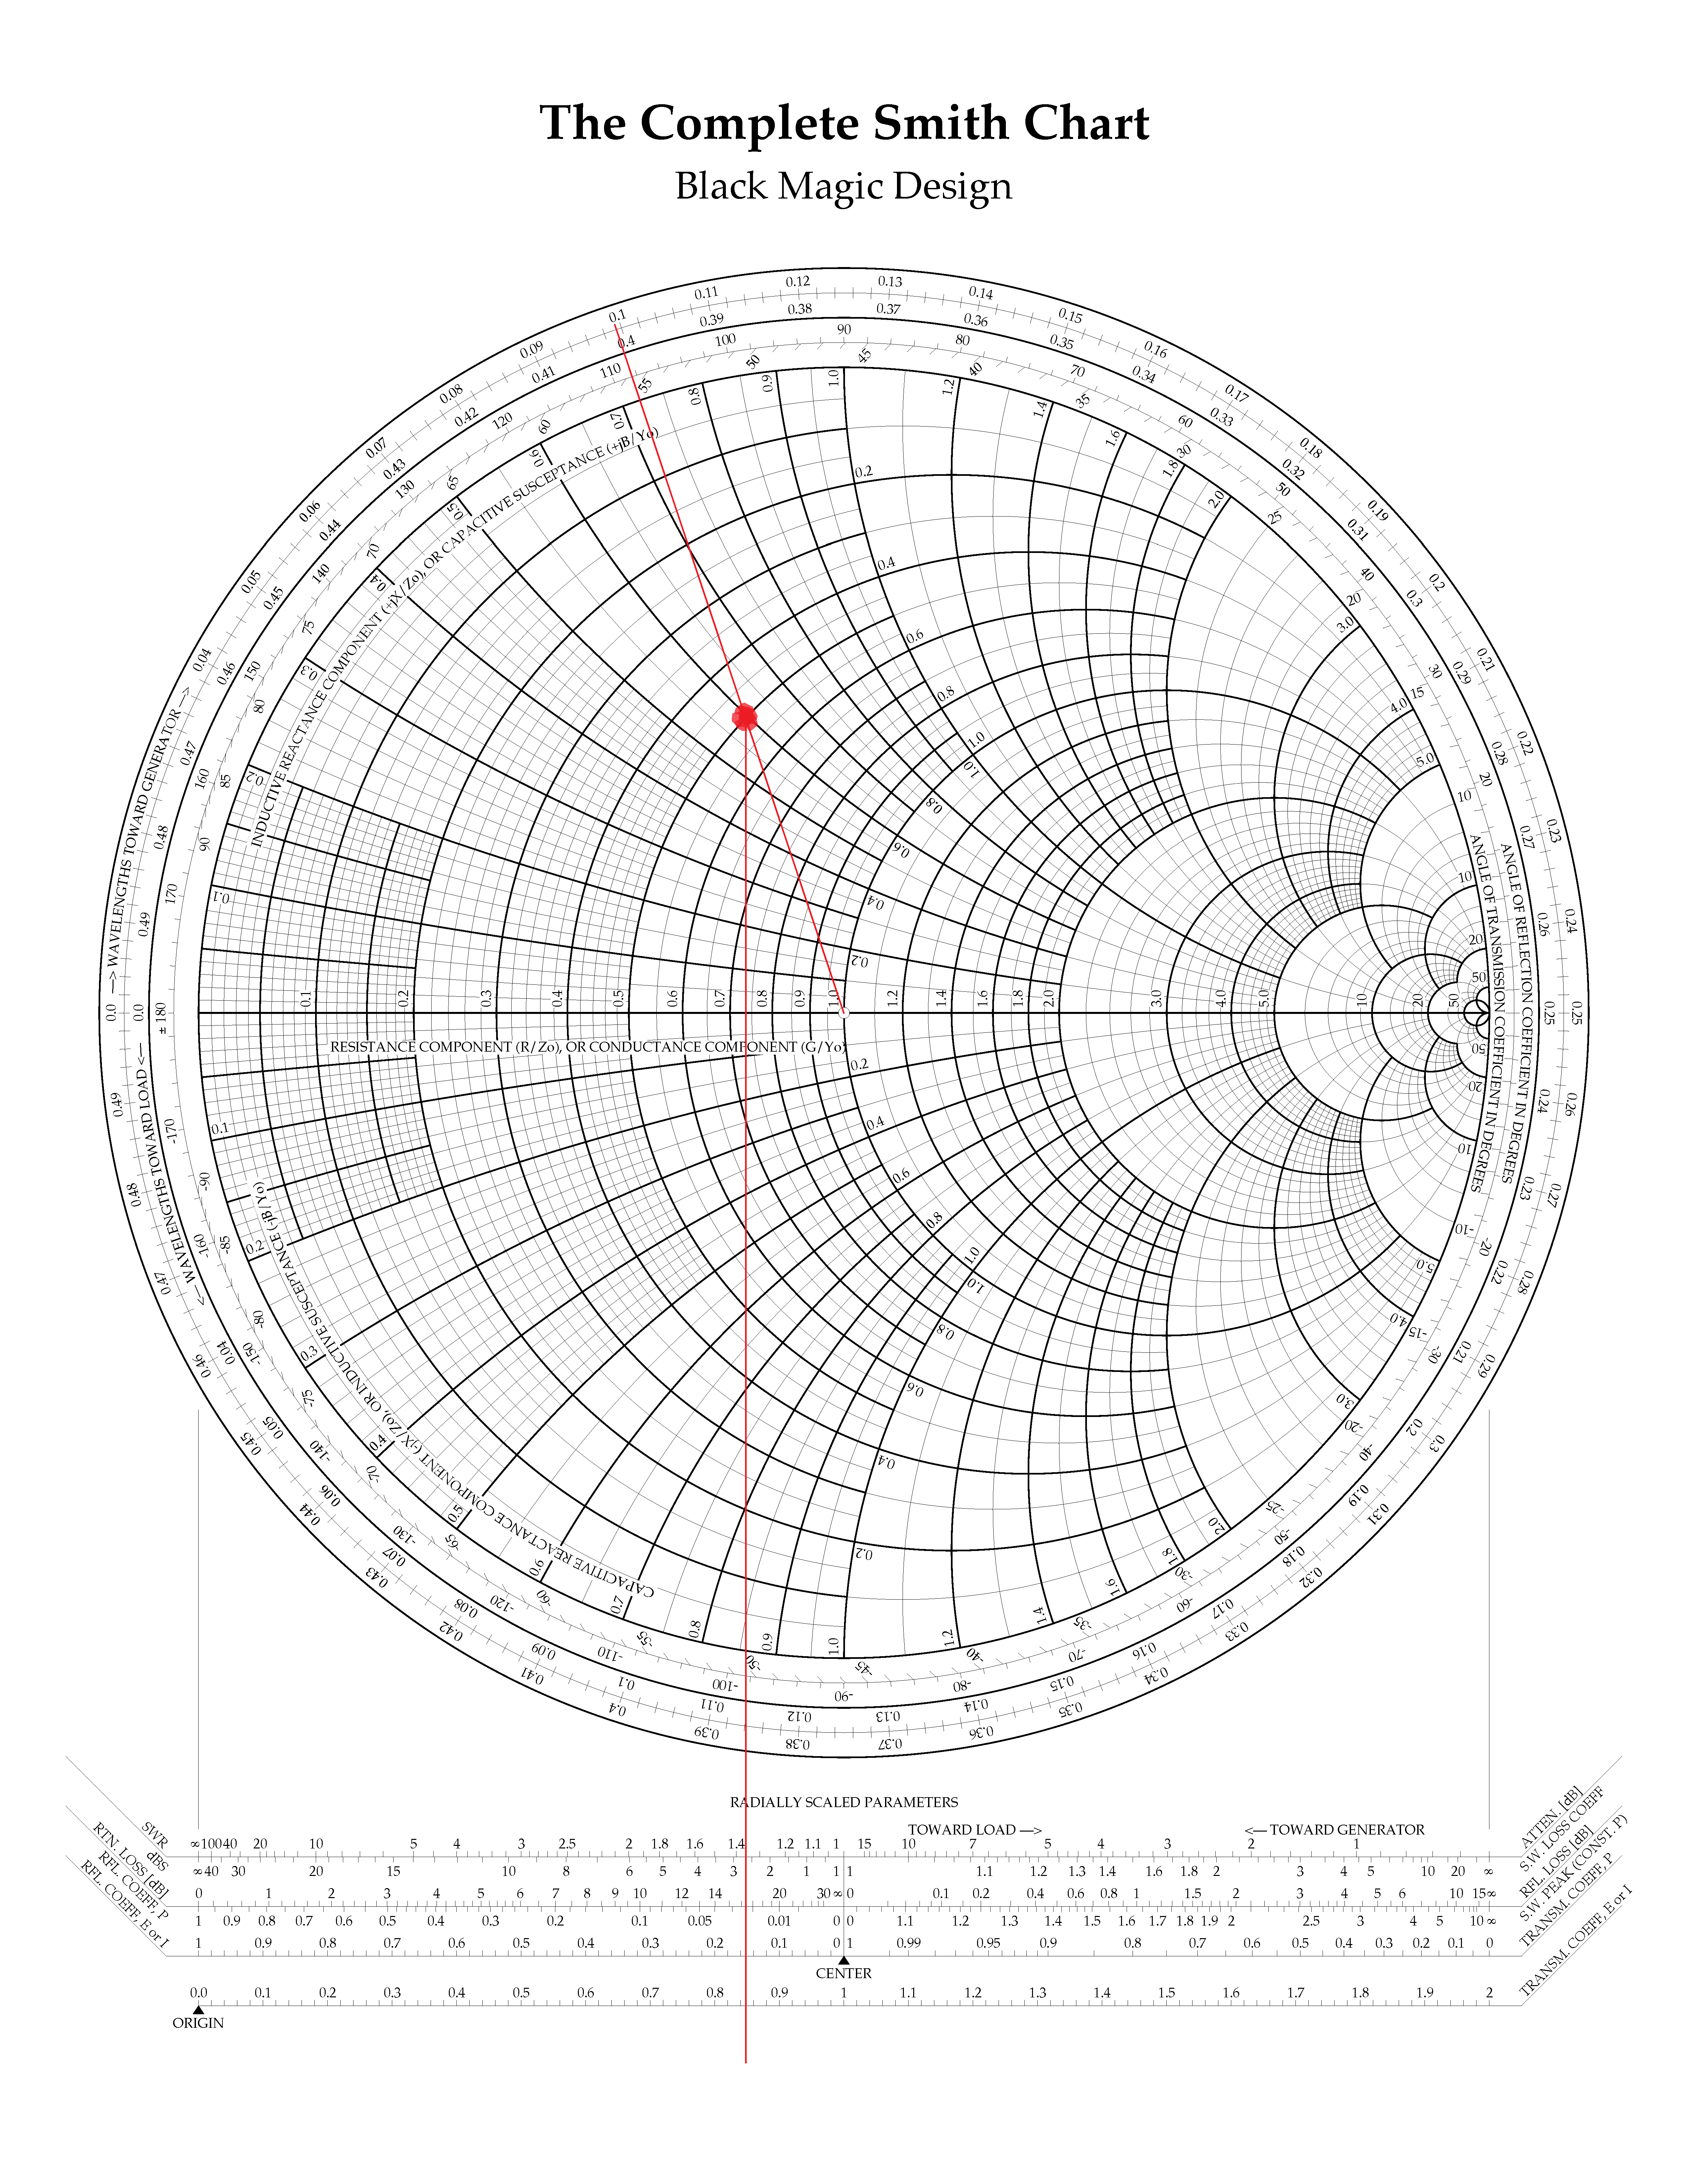
\includegraphics[height=8cm]{impedance_smith_chart.png}
    %\end{figure}

    We observe $|\rho_L| = 0.15$ and $phase(\rho_L) = 108.5 \deg$. Which translates to $\rho_L = -0.14158 + 0.42313j$. Pretty close.

    \item Assume $Z_0 = 50 \Omega$, use the Smith Chart to find the load impedance for $\rho_L = 0.5 + 0.1j$.

    \item Repeat (a) and (b) with $Z_0$ changed to $10\Omega$.

    \item For the following two circuits, trace $\rho_L$ on a Smith Chart with $Z_0 = 50\Omega$.

    \begin{figure}[H]
        \centering 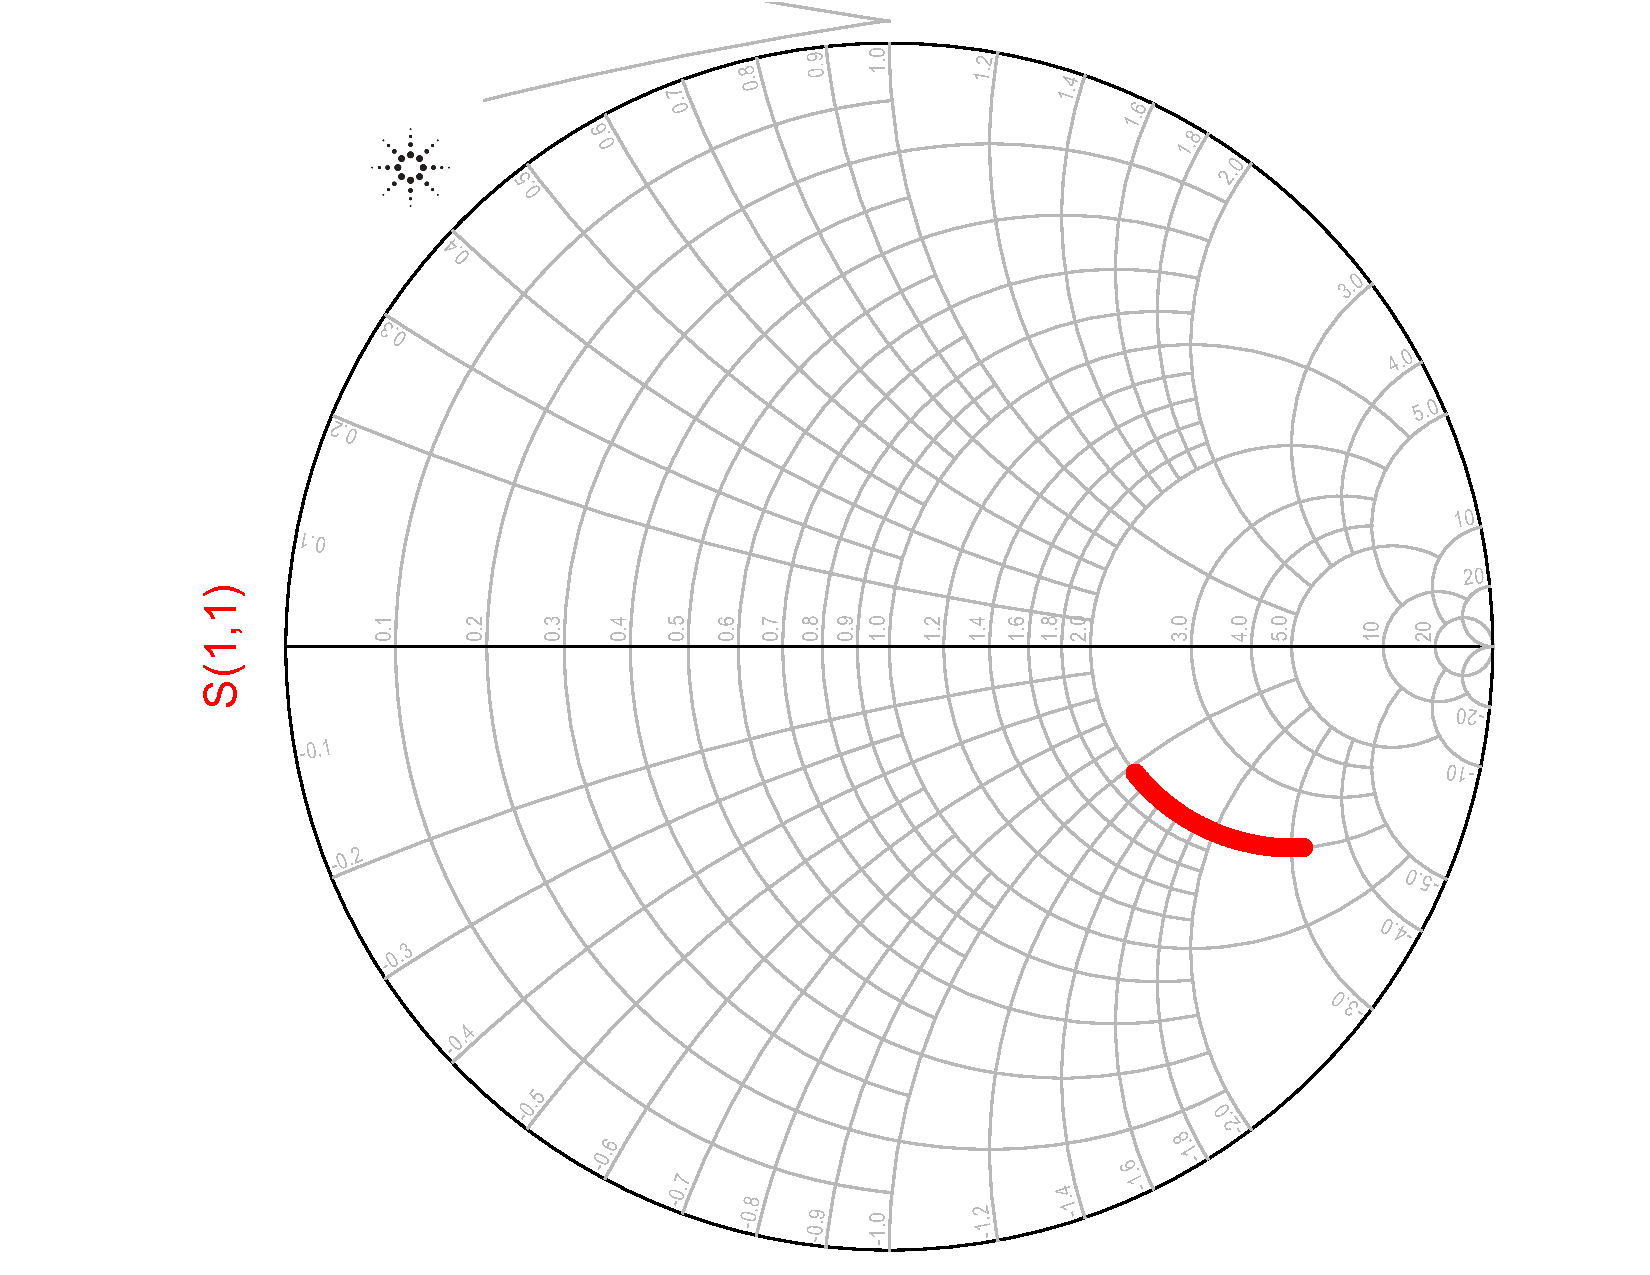
\includegraphics[width=\textwidth-9cm]{problem2d1.pdf}
        \centering 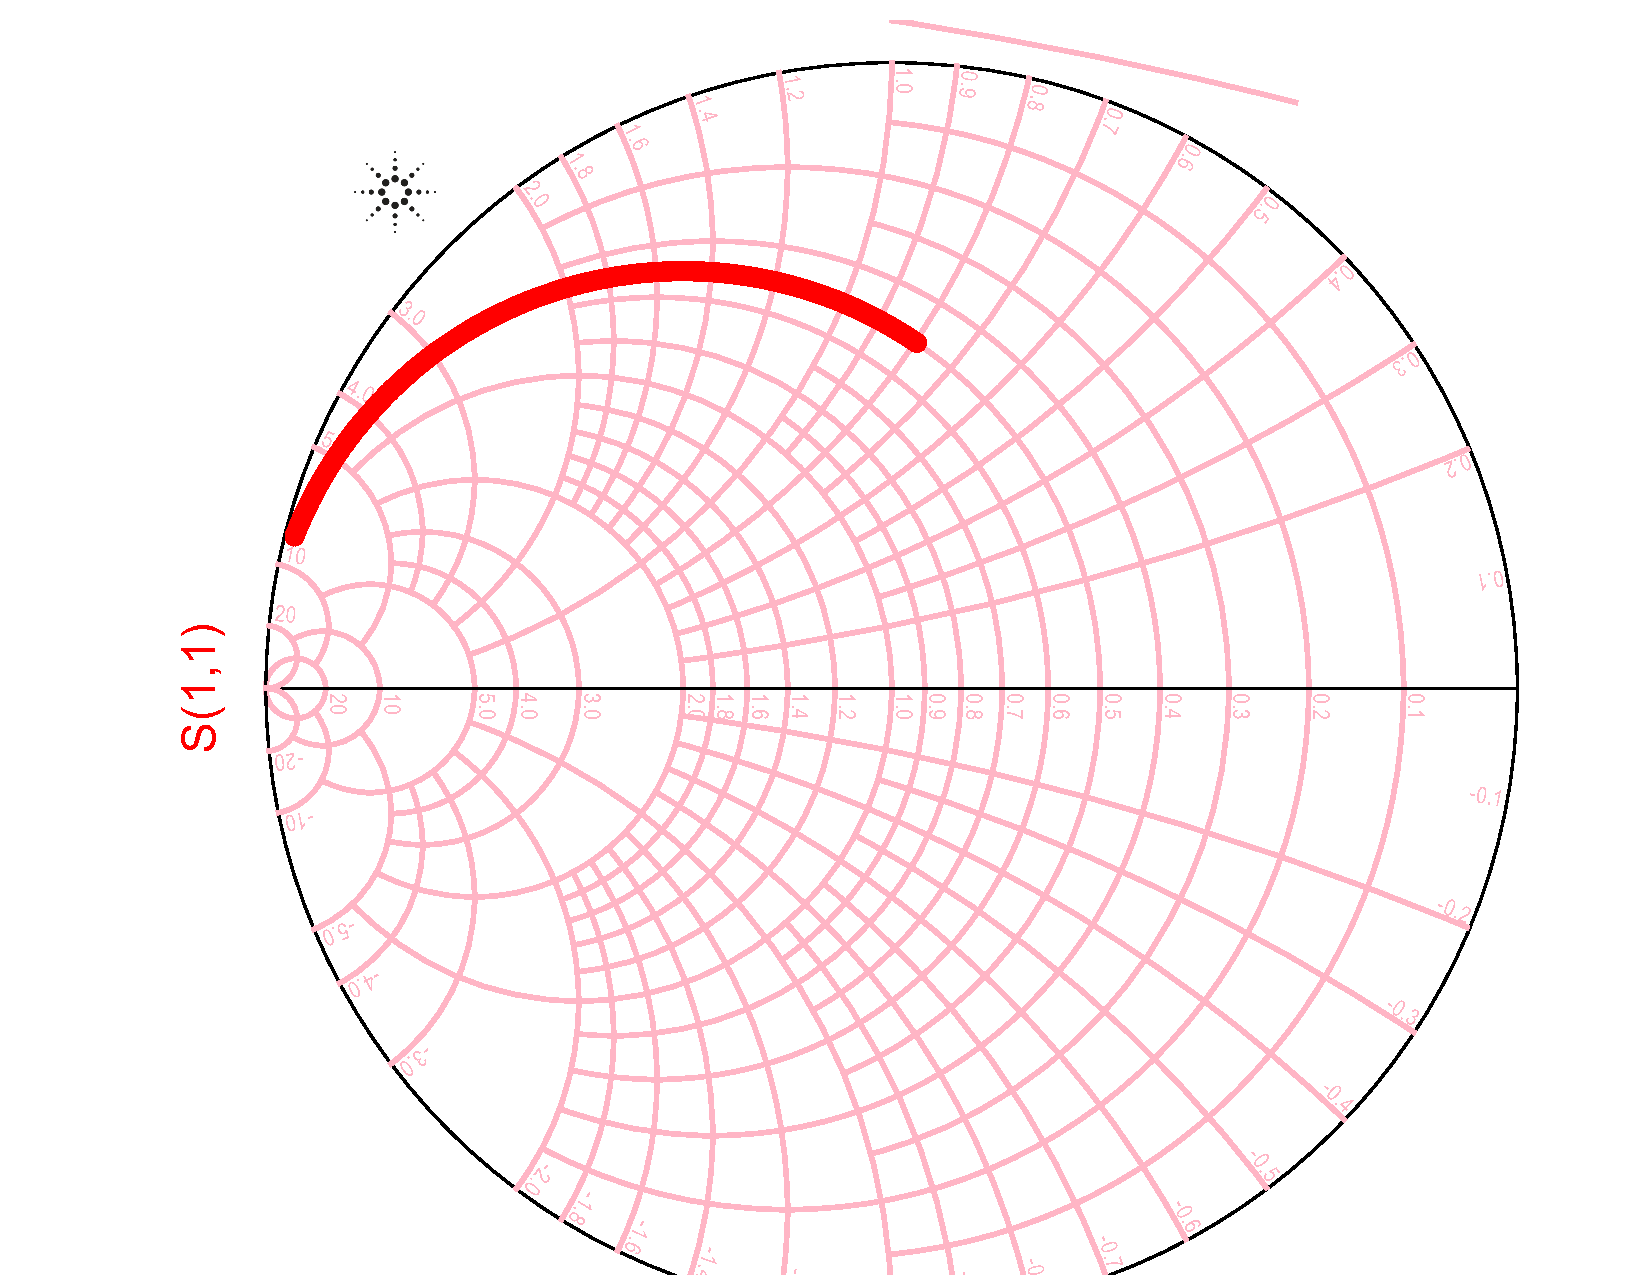
\includegraphics[width=\textwidth-9cm]{problem2d2.pdf}
    \end{figure}
\end{enumerate}

\section*{Problem 3}

\begin{enumerate}[label=(\alph*)]
    \item Assume $Y_0 = 0.02S$, use the Admittance Smith Chart to find the $\rho_L$ for a load impedance $Z_L = 25 + 30j \Omega$.

    \item Trace $\rho_L$ for the second circuit shown above with the parallel inductor, but on the admittance smith chart.
\end{enumerate}

\section*{Problem 4}

\begin{enumerate}[label=(\alph*)]
    \item What is the maximum power that can be extracted from the soure shown above? What is the load impedance for the max power delivery to happen?

    The maximum power transfer occurs when the (real) load impedance matches the (real) source impedance. In that case, $Z_L = 50 \Omega$ and the power delivered to the load is:
    \begin{align*}
        V_L &= \frac{1}{2} V_s \\
        I_L &= \frac{V_s}{100} \\
        P_{L,ac} &= \frac{V_s^2}{200 \cdot 2} = 2.5 \text{ mW}
    \end{align*}

    \item Drive a $500\Omega$ load. What is the power delivered and the load voltage?
    \begin{align*}
        V_L &= \frac{Z_s}{Z_s + Z_L} V_s = 0.091 \\
        I_L &= \frac{V_s}{500} = 2 \text{ mA} \\
        P_L &= 0.18 \text{ mW}
    \end{align*}

    \item Let's try to achieve impedance matching by putting a resistor in parallel with the load. What should the resistor value be and what is the actual power delivered to the load?
    \begin{align*}
        R_{match} || R_L = 50 \rightarrow R_{match} = \frac{50 R_L}{R_L - 50} &\rightarrow R_{match} = 55.5 \Omega \\
        V_{load,match} &= \frac{1}{2} V_s \\
        I_L = V_L/R_L = 1 \text{ mA} \\
        P_L = 0.5 \text{ mW}
    \end{align*}
    This approach doesn't work well since the maximum power is extracted from the load, but it is mostly wasted in the matching resistance.

    \item Design an impedance matching network using an ideal shunt capacitor and an ideal series inductor. What are the values?

    We start on the real impedance axis at 10. We move on a constant conductance circle to the -0.3j constant suspectance curve.
    This yields $C = \frac{0.3 / Z_0}{2 \pi \cdot 1e9} = 0.95$ pF.

    We then are on the constant resistance circle and can use a series inductor; we move on the 3j circle on the impedance chart.
    This yields $L = \frac{3 \cdot Z_0}{2 \pi \cdot 1e9} = 23.9$ nH.

    Simulation confirms that maximum power reaches the load.

    \item Calculate the load voltage and power.

        We model each leg as an impedance, with the first leg being $Z_s + j \omega L$ and the second $\frac{Z_L}{1 + j\omega C}$. Then $V_L$ can be found as a voltage divider and the same current goes through both legs. We find $Re(V_L) = 0.509 \text{ V}$, and $Re(I_L) = 10 \text{ mA}$, thus total power is maximized to the load at $P_L = 2.5 \text{ mW}$
\end{enumerate}
\end{document}
